\documentclass[a4paper]{IEEEtran}

  \usepackage{graphicx}
  \usepackage{hyperref}
  \usepackage{tabularx}
  \usepackage{multirow}
  \usepackage{tikz}
  \usepackage{pgfplots}
  
  \usepgfplotslibrary{statistics}
  
  \newcommand{\specialcell}[2][c]{%
  \begin{tabular}[#1]{@{}c@{}}#2\end{tabular}}
  
  \graphicspath{{illustrations/}}
  \pgfplotsset{compat=1.8}
  
  \pgfplotsset{
    /pgfplots/ybar legend/.style={
    /pgfplots/legend image code/.code={%
      \draw[##1,/tikz/.cd,yshift=-0.30em]
        (0cm,0cm) rectangle (3pt,0.8em);},
    },
  }
  
  \begin{document}
  
  \setlength{\tabcolsep}{10pt}
  \renewcommand{\arraystretch}{1.25}
  
  \begin{center}
    \textbf{\Large{
      Dragon Arena System: \\ A distributed multiplayer board game
    }}\\
    \vspace{0.25cm}
    \emph{Authors}: SB~Ramalingam Santhanakrishnan (4740270), \\ and Z~Sun () \\
    ICT Innovation, EEMCS, TU Delft\\
    \emph{Emails}: \{S.B.RamalingamSanthanakrishnan, Z.Sun-1\}@student.tudelft.nl\\
    \vspace{0.2cm}
    \emph{Course Instructors}: Jan S. Rellermeyer,\\
    PDS Group, EEMCS, TU Delft\\
    \emph{Email}: j.s.rellermeyer@tudelft.nl@tudelft.nl\\
    \vspace{0.2cm}
    \emph{Teaching Assistants}: L~Versluis and S~Talluri,\\
    EEMCS, TU Delft\\
    \emph{Emails}: {\{L.F.D.Versluis@, S.Talluri@student\}.tudelft.nl}\\
  \end{center}
  
  \vspace{0.2cm}
  
  \textbf{
    \emph{Abstract}---\emph{Dragon Arena System} (DAS) is an online multiplayer board game service designed for the specific requirements of WantGame BV, implemented as a distributed system. Multiple players from different locations coordinate on the virtual board to eliminate a strong AI adversary, namely the dragons. The service is hosted on Amazon Web Services (AWS) IaaS barebone compute resources, running in multiple instances to allow for scalability and fault tolerance and the system is written in NodeJS in functional reactive style. In our design, we prioritize availability and the overall responsiveness of the service while maintaining a reasonable consistency. We test the system using simulated client bots and show that the system can stay responsive under peak load to more than x\% of the clients and also analyze the fault tolerance capabilities of the system. 
  }
  
  \section{Introduction}
  
  WantGame BV is a popular online gaming company and are designing a new board game ready to roll out to multiple players. As the company is entering the rapidly expanding market of gaming, they face stiff competition and must maximize the user experience in order to survive in the industry, if not make profit. The gaming server must be able to cope up with peak traffic demands and frequent disconnections from players. Thus, WantCloud BV is evaluating several system designs for their brand new game engine, one of which is presented and analyzed in this report.
  
  The proposed system utilizes Amazon Web Services (AWS)~\cite{aws} IaaS cloud service provider's compute instance, EC2 (Elastic Cloud Compute) for providing on-demand compute capacity to host the game engine.
  Apart from using EC2, we do not depend on any other services provided by AWS so that WantGame BV can switch providers or self-host in the future. The gaming engine itself is written in NodeJS~\cite{nodejs}, on a single threaded event loop as it is a comfortable programming model for a gaming system (traditionally games have been written in while-true loops) and uses TCP/IP socket communication via websockets using the socket.io library~\cite{socket.io}. On the servers, the state is maintained on an immutable data store using the Redux library~\cite{redux} and async events are handled by the RxJS library~\cite{rxjs}. The gaming client is a small ReactJS~\cite{ReactJS} application which visualizes the board and allows keyboard inputs from the player. To simulate several players, we use client bot scripts which send simulated commands to the server, following a simple strategy to attack the dragons aggressively, events are logged both on the client and server side for later analysis.
  
  The overall system design follows the master-slave architecture, where the master server gets events directly from the clients directly connected to it and forwarded events from the clients connected to the slave servers. The master periodically broadcasts the current state of the system to all connected clients and slaves, which ultimately forward the state to their own connected clients.

  Prior work on designing gaming systems while maintaining consistency with efficient synchronization has been done in TSS~\cite{cronin2004efficient} with mirrored server architecture. We have adopted TSS to resolve late incoming events only on the master server. We have used disconnection log data from the Game Trace Archive~\cite{guo2012game}, specifically World of Warcraft's data and have scaled the timeline to our system for simulating client disconnection characteristics in our analysis. The goal of the test workload is to eliminate the AI units from the board.
  
  In \autoref{application}, additional background information on the application is provided. In \autoref{system_design} we illustrate the design of the system in detail with focus on specific aspects pertaining to WantGame's requirements and the rationale behind the decisions and tradeoffs that were considered. In \autoref{experiments} we present the experiments conducted along with the results and analysis. In \autoref{sec:discussion} we discuss our findings briefly and list potential improvements. We conclude the report in \autoref{conclusion} with a short summary on the main findings and recommendations to WantGame BV.
  
  \section{Application} \label{application}
  
  The online gaming server receives commands from end-users to act on their unit via the client application in a pre-agreed data protocol. The game comprises of a 25x25 board with two types of units, Knights (player) and Dragons (AI adversary). Knights can move, Dragons are static and the attack range is 2 squares, while the heal range is 5 squares distance, both non-diagonal distance and only Knights can heal each other. Each unit has health points and attack points, and aim to reduce the health of opponent units by attacking, which results in the opponent unit's reduction of health by the attacking unit's attack points. The system has been written in Typescript~\cite{typescript}, targeting NodeJS version 9 using ReactiveX extensions~\cite{reactivex}, ReduxJS~\cite{redux} for immutable state in the backend. The frontend and client bot have also been written in Typescript with ReactJS.
  
  \subsection{Requirements}
  
  In order to provide a reliable and interactive service, WantGame's requires the following aspects to be handled by the new system.
  
  \begin{itemize}
    \item \emph{Correct Operation}: At any point in the gameplay, the clients should see nearly consistent view of the board and actions applied on that state should be accommodated as far as possible, without violating the aforementioned rules of the game.
    \item \emph{Fault Tolerance and Availability}: The system should be resilient to failure of the clients and provide reasonable allowance for reconnection. Failure of a server instance should not result in overall seizure of the gameplay.
    \item \emph{Scalability}: The system should allow for connection of at least 100 players, supported by at least 5 functional servers.
    \item \emph{Responsiveness}: To allow for interactive gameplay, the system must remain responsive and update the board on the client as soon as the game reaches the new state.
    \item \emph{Monitoring}: At least two server instances should maintain a log of the events carried out. 
  \end{itemize}
  
  \begin{figure}[tbp]
    \centering
      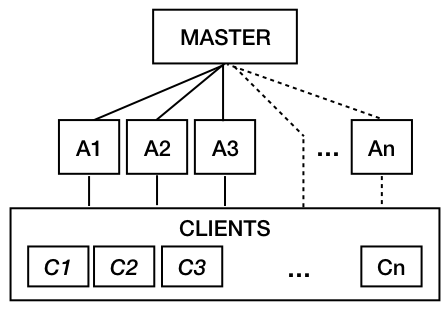
\includegraphics[width=\columnwidth]{system_design.png}
    \caption{Overview of system design.}
    \label{fig:overview_system_design}
  \end{figure}
  
  \section{System Design} \label{system_design}
  
  The master node accepts the commands from several clients and also the forwarded commands from slaves. The command is then carried out by the master at the timestamp mentioned in the command if not too old or by rolling back to that state and then replaying all commands that happened on that state following the requested command (determined by a policy). Periodically, the state updates are also sent back to the clients by the server, in turn forwarded by the agents to their own clients. Election of the master node is out of scope of the current implementation, thus we bootstrap the system with a pre-selected master and a list of successors. In the following sections we illustrate the components of the master and the overall working of the system in terms of consistency, synchronization, replication, fault-tolerance and availability.

  \subsection{Overview} \label{system_design_overview}
  
  The overall architecture of the system is illustrated in \autoref{fig:overview_system_design}, which can be seen consisting of a single master node, to which multiples agents, A1, A2, etc., are connected. Clients can connect to agents as well as the master directly, as far as the clients are concerned, the role of the server is opaque to them. Ideally, a load balancer is required in such architectures, however in this report we allow clients to randomly select servers from a known list and focus on other design aspects of the system. 
  
  The master node, illustrated in \autoref{fig:master_components} consists of the following components:
  
  \begin{itemize}
    \item \emph{Execution Queue}: The queue which maintains commands pending execution.
    \item \emph{Replay Set}: An ordered set (by timestamp) which holds the events that were previously executed, to support replays in the future. Older events in the set are periodically removed to recover memory. 
    \item \emph{Command Listener}: The socket server, which accepts client connections and subsequent commands, parses it, and adds it to the pending execution queue.
    \item \emph{Executor}: The core game engine loop present in master node which executes events in the execution queue, is invoked periodically (every 50ms in our case) and executes the event in the queue head.
    \item \emph{Broadcaster}: Broadcast the game state periodically (every 100ms in our case) to all the connected clients and agents. 
    \item \emph{Supervisor}: Responsible for logging all the actions executed in the system, deciding weather the current node is master/agent, self-election as master and maintaining connection with master.
  \end{itemize}

  Slave nodes differ from the master node in that they have a command forwarding component with a forwarding queue, instead of the executor, a state updating component connected to the master and the replay set is not utilized until it assumes the role of a master.
  
  \subsection{Working}
   
  \begin{figure}[bp]
    \centering
      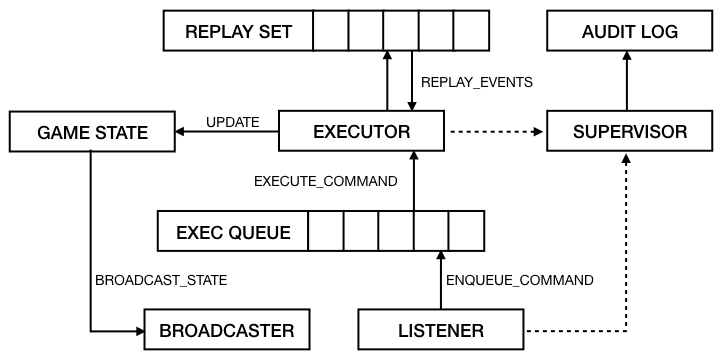
\includegraphics[width=\columnwidth]{master_components.png}
    \caption{Master components with message flows}
    \label{fig:master_components}
  \end{figure}
  
  The components in \autoref{fig:master_components} each have their own life cycle and associated events. Since we follow the reactive pattern, we illustrate the working of the system by tracing the through the execution of the system on receipt of a command from a client, through the system's various components.
  
  \begin{enumerate}
    \item \emph{Bootstrap}: This phase marks the start of the system, before the arrival of commands. The server nodes start and one of the nodes assumes leadership based on prior configuration and starts listening for client as well as agent connections. The game state consists of the board state with units and their health/attack points and also a scalar timestamp, set to 0 at the start. The timestamp is advanced on execution of each command. Agents make their connections to the master and listen for client connections as well as state updates from the master. 
  
    \item \emph{Command Receipt}: The listener listens for incoming commands from end-users and adds it to the execution queue. The executor periodically picks tasks from the execution queue, looks at the current timestamp and determines if the action can be executed on the current state if it is not too old (based on policy \textsc{Min\_Exec\_Window}), if above the policy window, it determines if the timestamp is below an executable window (policy, Max\_Exec\_Window) and attempts the rollback and execute operation illustrated in~\cite{cronin2004efficient}, provided the state is available in replay set. If the action is not executable at this point, it is simply discarded. If exists, then the executor picks the corresponding state from the replay set and executes all the stored commands that occurred after the given timestamp and finally updates the resultant state and also stores it in the replay state. We try to maintain weak consistency, on the assumption that most of the actions requested by the player are local to his/her position on the board, thus limiting the chances of overwriting other parts of the board. In case there are conflicting events, then we follow the policy of last-write wins. We do not differentiate actions leading to weak/strong consistency unlike in~\cite{cronin2004efficient}.

    \item \emph{Game State Progress}: As can be seen in command receipt handling, we try to make the best effort to accommodate as many client commands as possible for a point in time. But this could lead to stagnation of clients at some arbitrary timestamp until the server makes further progress due to rollbacks, which leads to more events queueing up in the same timestamp, leading to very slow or no progress at. To mitigate this, we do not send out any state updates or accept moves while the rollback is under execution. The slaves may still continue to accept actions from their own clients but they are dropped by the master until the rollback-replay is complete.

    \item \emph{Master Failover}: When the master fails, all of its connected clients attempt to connect to one of the other known servers. The slaves which were connected, recognize the event via socket disconnection. One of the slaves become a master and once the new master is alive, the master prioritizes all its buffered client commands first and then makes its best effort to execute the fresh forwarded commands. In case of drastic state changes, the clients which are connected to the agents will see a jump on their screens. It must be noted that the newly elected master is not aware of the replay set possessed by the previous master nor about its rollback/replay status, thus effectively everything is restarted from the last known stable state.

    \item \emph{Monitoring}: The role of the supervisor is to keep track of the executor and the listener. We explicitly log the execution queue each time an event is added to it, making the system repeatable to a large extent. We use the Bunyan~\cite{bunyan} library for formatting our log messages in Log4J~\cite{log4j} type of format.
 
  \end{enumerate}
  
  \subsection{System Capabilities \& Limitations}
  
  The major limitation of our architecture is that the clients connected directly to the master may enjoy better responsiveness if their connection paths offer lower latency compared to the clients connected to slaves. However, this could be mitigated by adding an artificial delay on the clients after a latency measurement step before spawning the units.
  
  \begin{enumerate}
    \item \emph{Synchronization, Consistency and Replication}: Synchronization and replication between the servers are pretty much achieved out of the box as a result of our architecture. We follow a weak consistency model, partly due to the fact that the game we are designing is not mission critical, contrary to LockStep~\cite{lockstep}, which would greatly reduce the responsiveness. Since we only guarantee weak consistency, we ensure the best effort to accommodate as many commands from a client as possible.

    \item \emph{Availability and Responsiveness}: Firstly, we make the system responsive by allowing clients to send commands asynchronously from the state updates. However, this could lead to inconsistent or updates made with a stale state assumption. This problem is mitigated by the mechanisms discussed in the previous sections. During failover, we continue to collect commands which makes the server available, but there is no guarantee if those messages will see light, unless the target server becomes the master.
  
    \item \emph{Fault Tolerance}: Our current implementation, can tolerate fail-stop on both the server as well as the client side. When a client fails, we wait for a timeout period until which if the player reconnects and claims the unit id, is allowed to continue, else the unit is removed from the board (\textsc{Unit\_Remove\_Timeout}).

  \end{enumerate}
  
  \section{Experimental Results} \label{experiments}
  
  We conduct a total of 3 experiments and analyse the results in the following sub-sections.
  
  \subsection{Setup}
  
  The goal of the experiments is to analyse the impact of consistency and responsiveness as a function of total client connections and disconnection events. The test system is deployed on the AWS cloud platform using bare bone EC2 compute instances. We use the m3.medium type (vcpus=1, memory=3.75Gb based on Intel Xeon E5-2670 v2) for both the master and the agent nodes. We restricted the deployment to a single region, North Virginia (US-East-1) with default availability zone placement policy and the default virtual private cloud settings provided by AWS. A custom security group is used for exposing corresponding ports to clients and agents.   

  The workload consists of client bots, managed by a runner which kills and spawns new bots as per the game trace archive's logs. The logs are recorded on the local AWS disk and analysed separately.
  We use python libraries pandas, scipy and numpy to analyse the time series log data and matplotlib for visualizing the same. We also run the bots on the same AWS region and availability zone subnet on a separate EC2 instance to minimize network disruptions.
  
  \subsection{Experiments}
  
  \subsubsection{Overheads}

  The latency between EC2 servers was found to be an average of x. Logging overhead was found to be y. To measure client consistency, we make them send the their board state explicitly back to the server at random timestamps, this leads to an extra command, which is however just for logging purposes but not executed by the server, leading to a negligible overhead. We did not find any other significant overheads that could affect the experiments on the client bot or any other part of the system.
  
  \subsubsection{Consistency Deviation}

  The metric for consistency deviation is the number of differences in the board position at a given timestamp. In order to measure this, the clients send their board state at some past timestamp and the server compares the received board with its own board at the same timestamp and logs the deviation.
  
  \subsubsection{Responsiveness}

  The metric for responsiveness is the timestamps taken for the server to accept the client's command, sent at timestamp t. We measure this on the client side by checking the received board state and see if the expected change occurred. We restrict our measurements to consider move commands only because it is difficult to ascertain the same for attack and heal if any other player unit's action had affected the state. This is acceptable, considering that move command makes up the majority of the commands. 
  
  \subsubsection{Fault tolerance}

  HOW TO GO ABOUT THIS? GAME TRACE ARCHIVE?

  \subsection{Server connection Benchmark}

  In order to aid future decisions on load balancing, network and other hardware capacity, we benchmark the a single server instance running on an EC2 instance on the number of socket connections that it can handle. We measure the memory and cpu load using NodeJS standard libraries as a function of clients connected. For this experiment, the AI dragons were disabled and the board size was expanded to 100x100 to accommodate as many clients as possible.
  
  \section{Discussion}
  
  \label{sec:discussion}
  
  The experiments and analysis suggest that....
  
  For future work on the implementation, we would like to work and present on a more accurate time
  series analysis to trace the events and identify patterns which lead to the specific problems
  we encountered with the current system. In addition we would like to work extensively to improve in the following areas.
  
  \begin{enumerate}
    \item Master restart and detecting network partition. Currently, only fail-stop of master node is supported.
    \item Scale up and scale down server instances dynamically. This is mainly to save cost but requires a leader election algorithm in place.
    \item Implement a load balancer so that the client connections are distributed fairly and low latency servers are selected by the clients. 
    \item Build replication and synchronization for hosting multiple masters. A simple addition could be to add a master to manage a separate region of the game map.
  \end{enumerate}
  
  Clearly there are many other drawbacks in our implementation which we wish to overcome. However the experiments gave deep insights into the various tradeoffs in building a distributed system which has tight constraints on responsiveness.
  
  \section{Conclusion} \label{conclusion}
  
  In the report, we have designed and analysed a multiplayer gaming engine, aligned to the chief requirement of WantGame BV, to maintain responsiveness at peak traffic demands, which is clearly met by the system, as seen in the experimental results, where a majority of the clients are able to see their action executed in under \textbf{x} (seconds), while maintaining a consistent view of the game. The tradeoff made in fault-tolerance and scalability has to be noted though, mainly in that the system is not elastic and has to have scaling mechanism in place without disruption of gameplay. In addition we found that in some cases, optimistically processing commands in the client and agent can greatly improve the responsiveness as well as offload the master server. After analyzing the tradeoffs, we think that it is a worthy endeavour for WantGame BV to build a system with the proposed design and keep improving as new features are to be met.
  
  \bibliographystyle{myIEEEtran}
  \bibliography{report}
  
  \section*{Appendix A: Time Sheets}
  
  \begin{table}[htbp]
    \centering
    \caption{Time spent on the project per activity.}
    \begin{tabular}{| l | c |}
      \hline
      Activity & Time (hours) \\
      \hline
      Total & 170 \\
      Think & 20 \\
      Dev & 80 \\
      XP & 15 \\
      Analysis & 15 \\
      Write & 20 \\
      Wasted & 20 \\
      \hline
    \end{tabular}
  \end{table}

  \begin{table}[htbp]
    \centering
    \caption{Time spent per experiment.}
    \begin{tabular}{| l | r | r | r |}
      \hline
      & \multicolumn{3}{| c |}{Time (hours)} \\
      \hline
      & Dev & Setup & Total \\
      \hline
      Consistency Deviation & 8 & 4 & 12 \\
      Responsiveness & 1 & 0.5 & 1.5 \\
      Fault Tolerance & 1 & 0.5 & 1.5 \\
      Benchmark & 1 & 0.5 & 1.5 \\
      \hline
    \end{tabular}
  \end{table}
 
  \end{document}